%\documentclass[letterpaper]{article}
\documentclass[12pt,letterpaper]{article}
\usepackage{amsmath, geometry, graphicx, tikz}
\usetikzlibrary{arrows.meta}
\bibliographystyle{plain}

\setlength{\textwidth}{480pt}
\setlength{\textheight}{630pt}
\setlength{\voffset}{0pt}

\title{Variation of Genomic Imprinting in the Human Brain}
%\title{Regulators and Psychiatric Associates of Genomic Imprinting in the Human Brain}
\author{Attila Guly\'{a}s-Kov\'{a}cs\(^\ast\), Ifat Keydar\(^\ast\),
...,
%\\
%Eva Xia, Menachem Fromer, Doug Ruderfer,\\
%Ravi Sachinanandam,
Andrew Chess}
\date{Mount Sinai School of Medicine}

\linespread{1.2}

\begin{document}

\maketitle

\begin{abstract}
We present the first genome-wide analysis of human genomic imprinting based on
RNA-seq measurements of the parental bias in allele-specific expression in the
dorsolateral prefrontal cortex.  We find that the fraction of imprinted human
genes is consistent with lower (\(\approx 0.5\%\)) as opposed to higher
(\(\approx 5\%\)) estimates in mice.  Our analysis reveals that age up or
down-regulates allelic bias of some imprinted genes even in later life and
that allelic bias depends also on gender and genetic variation.  Furthermore,
we show that allelic bias of some imprinted genes, like UBE3A in the
Prader-Willi region, is linked to schizophrenia.  These results support the
hypothesized role of imprinted genes in social interactions, which dynamically
change in the life course and depend on neuropsychological function.
\end{abstract}

\section{Introduction}

Genomic imprinting, leading to repression of either the maternal or paternal
allele, has reached its highest prevalence in humans and other placental
organisms~\cite{Renfree2012}.  In line with this, well-known physiological
functions of imprinted genes include embryonic and placental development, body
growth, suckling, and maternal behavior~\cite{Plasschaert2014,Peters2014}.
Genomic imprinting requires the placement of different epigenetic marks, such
as DNA methylation, at the respective alleles residing on the chromosomes
originating from the mother or father~\cite{Plasschaert2014}.  Indeed,
imprinted genes typically reside in clusters spanning hundreds of kilobases
and allele-specific differential epigenetic marks are found near specific
genes as well as in shared regulatory elements called imprinting control
regions. For non-imprinted genes expression is balanced such that the two
alleles are roughly equally expressed. By contrast, for imprinted genes
epigenetic marks lead to substantial, degrees of
imbalance in the expression level of the two alleles.  We refer to the degree
of expression imbalance as \emph{allelic bias}; at its maximum expression is
completely monoallelic.

Why natural selection favors allelic bias for imprinted genes remains
debated~\cite{Wilkins2003,McDonald2005,Keverne2015} but the most mature of all
theories, kinship or conflict theory~\cite{Wilkins2003}, provides a flexible
framework for interpreting past studies on imprinted genes and formulating
hypotheses and predictions regarding their detailed regulation and
physiological function.  The theory assumes that all imprinted genes contribute to
inter-individual interactions in a highly dose-dependent fashion, and explains
allelic bias with the conflicting interests of paternal and maternal genes,
which arise from sexual asymmetries in those interactions~\cite{Wilkins2003}.
A well-known asymmetry is the disproportionate role of mothers in
nurturing offspring in Placentalia.  Kinship theory thus explains why
overexpression disorders of paternally or maternally biased genes in children
abnormally promote or inhibit, respectively, their
growth~\cite{Plasschaert2014,Peters2014}.

Since different inter-individual interactions take place in various
developmental stages and are mediated by various organs, kinship theory
explains the non-uniform pattern of ``imprintedness'' and allelic bias over
various ages~\cite{Bourke2007} and tissue types, which is seen for several
imprinted genes~\cite{Plasschaert2014,Peters2014}.  For other genes such
patterns await discovery.  The theory quantitatively predicts relaxation of
allelic conflict with age~\cite{Ubeda2012} and so raises the hypothesis that
change in allelic bias is linked to aging.  A study on newborn and young adult mice
partially supports that hypothesis~\cite{Perez2015} but experimental evidence
from humans, including older individuals, is missing.

In the framework of kinship theory the question of aging is closely tied to
the roles of imprinted genes in social interactions and in the underlying
psychiatric functions~\cite{Ubeda2012,Wilkins2003}, whose importance has been
increasing in human evolution.  Indeed, most human imprinted gene syndromes
are characterized by not only growth disorder but also mental retardation and
psychiatric dysfunction~\cite{Plasschaert2014,Peters2014}.  More precisely,
paternally and maternally biased genes are suggested to play antagonistic
roles not only in growth but also in psychiatric functions~\cite{Crespi2008a},
since overexpression of the former is associated with autistic while that of
the latter with psychotic spectrum disorders.  For example, maternally derived
microduplications at 15q11-q13 may not only cause the Prader-Willi
syndrome~\cite{Peters2014}---whose symptoms include obesity---but also highly
penetrant for schizophrenia~\cite{Ingason2011,Sullivan2012}, which is perhaps the most devastating
psychotic spectrum disorder.

Recently the CommonMind Consortium produced and
shared\footnote{www.commonmind.org} genome-wide data sets on genotype and gene
expression in the dorsolateral prefrontal cortex (DLPFC) of hundreds of
schizophrenic and control individuals, and identified some 650 differentially
expressed genes~\cite{Fromer2016a}. Our present work extends that analysis
with a focus on allele-specfic expression across the genome, allowing us to
determine allelic bias for each gene.  Based on that, we find that \(\approx
0.6\%\) of all genes are imprinted in the human DLPFC, the majority of which
had been reported to be imprinted in the context of one or another tissue
and/or species. We find a number of genes with allele specific expression
residing near clusters of known imprinted genes. Furthermore, our data suggest
that for several imprinted genes the variation of allelic bias across
individuals is explained by differences in age, schizophrenia diagnosis,
gender or ancestry.  For example, UBE3A in 15q11-q13, appears to have
allele-specific bias that varies with age and psychiatric condition.

\section{Methods}

\subsection{Study design}

We used allele-specific RNA-seq read counts from the CommonMind project to
probe the allelic bias of expression for each gene \(g\) that is
substantially expressed in the DLPFC.  We exploited the fact that single
nucleotide polymorphisms (SNPs) provide a way to distinguish between the two
parental alleles.  For a heterozygous SNP \(s\) in a gene the reference and the
alternative variant tags the maternal and paternal allele or the other way
around.  When allelic bias towards positively biased allele \(b\) (which may
be maternal or paternal) is strong then it seems likely that the count of
reads tagged by the corresponding SNP variant (which may be reference or
alternative) is also relatively high.

This intuition may be formalized by introducing \(p\), the fraction of
transcripts from the parent towards which expression is biased.  \(p\) is
interpretable as the strength of allelic bias.  Note that \(1/2\le p\le 1\).
Let \(b\) identify the positively biased allele, i.e.~the allele with the
higher number of transcripts.  Now let \(B\) denote the count of RNA-seq reads
that map to the \(b\) allele at a SNP that distinguishes \(b\) from the other
allele.  Similarly, let \(T\) denote the total read count at that SNP.  Then,
assuming that \(B\) is a binomial random variable with given denominator \(T\)
and expected relative frequency \(p\), the probability that \(B\) is the
higher of the two read counts, i.e.~\(B \ge T - B\), is \[\sum_{x:T/2\le x\le
T} {T \choose x} p^x (1 - p)^{T-x}.\] The fact that this probability increases
with \(p\)---as allelic bias gets stronger---supports our intuition.

These considerations motivated us to quantify allelic bias using a statistic called
\emph{read count ratio} \(S\), whose definition we
based on the total read count \(T\) and the \emph{higher read count} \(H\),
i.e.~the count of reads carrying only either the reference or the alternative SNP variant,
whichever is higher.  The
definition is
\begin{equation}
S_{ig} = \frac{H_{ig}}{T_{ig}}= \frac{\sum_s H_s}{\sum_sT_s},
\label{eq:S-definition}
\end{equation}
where \(i\) identifies an individual, \(g\) a gene, and the summation runs
over all SNPs \(s\) for which gene \(g\) is heterozygous in individual \(i\) (Fig.~\ref{fig:study-design}).
Note that if \(B_{ig}\) is the count or reads that map to the \(b_{ig}\) allele
(defined as above) and if we make the same distributional assumption as above, namely that \(B_{ig}\sim
\mathrm{Binom}(p_{ig}, T_{ig})\), then \(\mathrm{Pr}(H_{ig}=B_{ig}|p_{ig})\), the probability of correctly
assigning the reads with the higher count to the allele towards which
expression is biased, tends to 1 as \(p_{ig} \rightarrow 1\).  We took
advantage of this theoretical result in that we subjected only those genes to
statistical inference, whose read count ratio was found to be high and,
therefore, whose \(p_{ig}\) is expected to be high as well.

Fig.~\ref{fig:study-design} illustrates the calculation of \(S_{ig}\) for the
combination of two hypothetical genes, \(g_1,g_2\), and two individuals,
\(i_1,i_2\).  It also shows an example for the less likely event that the lower rather
than the higher read count corresponds to the SNP variant tagging the higher
expressed allele (see SNP \(s_3\) in gene \(g_1\) in individual \(i_2\)).

Using the read count ratio we analyzed two aspects of the variation of allelic
bias.  First, we ranked all expressed genes according to the \emph{gene
score}, a summary statistic that quantifies how right-shifted the distribution
of \(S_{ig}\) is for any given gene \(g\), and combined that information with
prior evidence for imprinting.  Second, given a top-scoring gene \(g\), we
sought to identify biological regulators and psychiatric consequences of
allelic bias by studying the conditional distribution of \(S_{\cdot g}\) given
observations \(x_{\cdot 1},...,x_{\cdot p}\) on features of study individuals
that are not gene-specific. We call these features \emph{predictors} because
we used them in a regression model framework.  Predictors and their various
levels (if any) are listed in Table~\ref{tab:predictors}.

Before we carried out our read count ratio-based analyses, however, we cleaned
our RNA-seq data by quality-filtering and by improving the accuracy of SNP
calling with the use of DNA SNP array data and imputation. In the following
subsections of Methods we describe the data, these procedures, as well as our
regression models in detail.

\subsection{Data}

\subsubsection{Brain samples, RNA-seq}

Human RNA samples were collected from the dorsolateral prefrontal cortex of
the CommonMind consortium from a total of \(579\) individuals after
quality control. Subjects included 267 control individuals, as well as 258
with schizophrenia (SCZ) and 54 with affective spectrum disorder (AFF).
RNA-seq library preparation uses Ribo-Zero (which selects against ribosomal
RNA) to prepare the RNA, followed by Illumina paired end library generation.
RNA-seq was performed on Illumina HiSeq 2000.

\subsubsection{Mapping, SNP calling and filtering}

We mapped 100bp, paired-end RNA-seq reads (\(\approx50\) million reads per sample) using Tophat
to Ensembl gene transcripts of the human genome (hg19; February, 2009) with
default parameters and 6 mismatches allowed per pair (200 bp total). We
required both reads in a pair to be successfully mapped and we removed reads
that mapped to \(>1\) genomic locus. Then, we removed PCR replicates using the
Samtools rmdup utility; around one third of the reads mapped (which is
expected, given the parameters we used and the known high repeat content of
the human genome). We used Cufflinks to determine gene expression of Ensembl
genes, using default parameters. Using the BCFtools utility of Samtools, we
called SNPs (SNVs only, no indels). Then, we invoked a quality filter
requiring a Phred score \(>20\) (corresponding to a probability for an
incorrect SNP call \(<0.01\)).

We annotated known SNPs using dbSNP (dbSNP 138, October 2013). Considering all
579 samples, we find 936,193 SNPs in total, 563,427 (60\%) of which are novel.
Further filtering of this SNP list removed the novel SNPs and removed SNPs
that either did not match the alleles reported in dbSNP or had more than 2
alleles in dbSNP. We also removed SNPs without at least 10 mapped reads in at
least one sample. Read depth was measured using the Samtools Pileup utility.
After these filters were applied, 364,509 SNPs remained in 22,254 genes. These
filters enabled use of data with low coverage.  For the 579
samples there were 203 million reads overlapping one of the
364,509 SNPs defined above.  Of those 158 million (78\%) had genotype data
available from either SNP array or imputation.

\subsubsection{Genotyping and calibration of imputed SNPs}

DNA samples were genotyped using the Illumina Infinium SNP array. We used
PLINK with default parameters to impute genotypes for SNPs not present on the
Infinium SNP array using 1000 genomes data.  We calibrated the
imputation parameters to find a reasonable balance between the number of genes
assessable for allelic bias and the number false positive
calls since the latter can arise if a SNP is
incorrectly called heterozygous.

We first examined how many SNPs were heterozygous in DNA calls and had a
discordant RNA call (i.e.~homozygous SNP call from RNA-seq) using different imputation
parameters. Known imprinted genes were excluded. We examined RNA-seq reads
overlapping array-called heterozygous SNPs which we assigned a heterozygosity
score \(L_\mathrm{het}\) of 1, separately from RNA seq data
overlapping imputed heterozygous SNPs, where the \(L_\mathrm{het}\) score could
range from 0 to 1.  After testing different thresholds
we selected an \(L_\mathrm{het}\) cutoff of 0.95 (i.e. imputation confidence
level of 95\%), and a minimal coverage of 7 reads per SNP. With these
parameters, the discordance rate (monoallelic RNA genotype in the context of a
heterozygous DNA genotype) was 0.71\% for array-called SNPs and 3.2\% for
imputed SNPs.

The higher rate of discordance for the imputed SNPs
is due to imputation error.  These were taken into
account in two ways.
First, we considered all imputed SNPs for a gene \(g\) and individual \(i\)
jointly.  Second, we excluded
any individual, for which one or more SNPs supported biallelic
expression.

%At this point, the matrix includes 147
%million data points covering 213,208 SNPs, of which 114 million (77\%) have
%imputation data.

\subsubsection{Quality filtering}

\label{sec:filtering}

Two kind of data filters were applied sequentially: (1) a \emph{read
count-based} and (2) an \emph{individual-based}.  The read count-based filter
removes any such pair $(i,g)$ of individual $i$ and genes $g$ for which the
total read count $T_{ig}<t_\mathrm{rc}$, where the read count threshold
$t_\mathrm{rc}$ was set to 15. The individual-based filter removes any genes
$g$ (across all individuals) if read count data involving $g$ are available
for less than $t_\mathrm{ind}$ number of individuals, set to 25.
These final filtering procedures decreased the number of genes in the data from
\(15584\) to \(n=5307\).

\subsection{Statistical analysis}

\subsubsection{Test for nearly unbiased expression}

This test was defined by the criterion
\begin{equation}
S_{ig} \le 0.6 \text{ and } \mathrm{UCL}_{ig} \le 0.7,
\label{eq:unbiased-test}
\end{equation}
where the 95\% upper confidence limit \(\mathrm{UCL}_{ig}\) for the expected
read count ratio \(p_{ig}\) was calculated based on the assumption
that the higher read count \(H_{ig}=S_{ig}T_{ig}\sim \mathrm{Binom}(p_{ig},
T_{ig})\), on the fact that binomial random variables are
asymptotically (as \(T_{ig}\rightarrow \infty\)) normal with
\(\mathrm{var}(H_{ig}) = T_{ig}p_{ig}(1-p_{ig})\), and on the equalities
\(\mathrm{var}(S_{ig}) = \mathrm{var}(H_{ig}/T_{ig}) =
\mathrm{var}(H_{ig})/T_{ig}^2\).  Therefore
\begin{equation}
\mathrm{UCL}_{ig} = S_{ig} + z_{0.975} \sqrt{\frac{S_{ig} (1 - S_{ig})}{T_{ig}}},
\end{equation}
where $z_{p}$ is the $p$ quantile of the standard normal distribution.

\subsubsection{Regression models}
\label{sec:methods-regression}

Let \(m\) denote the number of individuals/samples and \(\mathcal{G}\) the set
of \(n=5307\) genes that passed quality filtering.  Regression analysis
involved a subset \(\mathcal{G}_1\subset\mathcal{G}\) of \(n_1=30\) genes
called as imprinted.

The basic model, unlm.S, is
\begin{eqnarray}
\mathbf{S} &=& \mathbf{X} \boldsymbol{\beta} + \boldsymbol{\varepsilon},
\label{eq:unlm.S-matrix-form} \\
\varepsilon_{ig} &\overset{\mathrm{iid}}{\sim}& \mathrm{Norm}(0, \sigma^2_g)
\end{eqnarray}
where the response \(\mathbf{S}\) is an \(m\times n_1\) read count matrix with
entries \(S_{ig}\), \(\mathrm{X}\) is an \(m\times p\) design matrix,
\(\boldsymbol{\beta}\) is a \(p\times n_1\) matrix of regression
coefficients~(Table~\ref{tab:predictors}), the random error
\(\boldsymbol{\varepsilon}\) has the same dimension as \(\mathbf{S}\), and
gene \(g\in \mathcal{G}_1\).  Eq.~\ref{eq:unlm.S-matrix-form} may be given as
\begin{equation}
S_g = \mathbf{X} \beta_g + \varepsilon_g,
\label{eq:unlm.S-vector-form}
\end{equation}
where the vectors \(S_g, \beta_g, \varepsilon_g\)
are single columns taken from their respective matrix counterparts.

The unlm.S model was extended in several ways, yielding
\begin{enumerate}
\item six normal linear models (Table~\ref{tab:nlm})
\item two logistic models logi.S and logi2.S.
\end{enumerate}

The general form of the normal linar models
(cf.~\ref{eq:unlm.S-vector-form}) is
\begin{equation}
\mathbf{W}_g^{1/2} \tau(S_g) = \mathbf{W}_g^{1/2} \mathbf{X} \beta_g + \varepsilon_g.
\label{eq:nlm-general}
\end{equation}
The extension here consists of \(\mathbf{W}_g\), an \(m\times m\) diagonal matrix of
weights \(w_{ig}\) on the \(i\)-th diagonal position, and \(\tau\), a
transformation on read counts.  Besides the trivial identity transformation
(i.e.~no transformation) two kinds of transformation were used: the rank
transformation and a quasi-log transformation \(\tau_Q\) defined as
\begin{equation}
\tau_Q(S_{ig};T_{ig}) \equiv Q_{ig} = - \log \left( 1 - S_{ig} \frac{T_{ig}}{T_{ig} + c}
\right),
\label{eq:Q}
\end{equation}
where \(\log\) means natural logarithm (base \(e\)).  \(c\) is a pseudo read
count set to \(1\) in order to avoid zero in the parenthesis since the \(\log\)
function is undefined at \(0\).

The logistic models, logi.S or logi2.S, share the general form
\begin{eqnarray}
S_g &=& \mu_g + c\, \varepsilon_g
\label{eq:logi-general}
\\
\mu_g &=& h(\mathbf{X} \beta_g)
\label{eq:glm-mean-predictor}
\\
\varepsilon_{ig} + \mu_g &\overset{\mathrm{iid}}{\sim}& \mathrm{Binom}(\mu_g, T_{ig}).
\label{eq:binom-error}
\end{eqnarray}
The link function \(h\) is \(h(u) = e^u / (1 + e^u)\) for logi.S and \(h(u) =
e^u / (2 + 2e^u)] + 1/2\) for logi2.S, and the scaling constant \(c\) is 1
 and \(1/2\), respectively.  Thus, the response \(S_g\) under logi2.S is scaled and shifted relative to
that under logi.S such that (with probabilty one) \(1/2\le S_{ig}\le 1\) under the former and
\(0\le S_{ig}\le 1\) under the latter.

Each of the eight models (including normal linear and logisitc models) has \(p\times n_1\) regression parameters corresponding to the
dimension of \(\boldsymbol{\beta}\).  This allows different behavior for
different genes since \(\beta_1\neq ...\neq\beta_{n_1}\) in general.
Therefore, the estimated regression coefficients are reported as \(\hat{\beta}_g =
(\hat{\beta}_{1g},...,\hat{\beta}_{jg},...,\hat{\beta}_{pg})\) for each gene \(g\), often
replacing index \(j\) with the name of the parameter such as \emph{Age} or
\emph{InstitutionPitt} (Table~\ref{tab:predictors}).

A second set of eight models was also
fitted, for which \(\boldsymbol{\beta}\) was constrained such that \(\beta_1 =
... = \beta_{n_1}\).  This was achieved by aggregating over genes
\(g\in\mathcal{G}_1\) the higher read count \(H'_i = \sum_g H_{ig}\), the
total read count \(T'_i = \sum_g T_{ig}\), redefining the read count ratio
as \(S'_i = H'_i / T'_i\), and replacing \(S_g\) by \(S'=(S'_1,...,S'_m)\) in
Eq.~\ref{eq:unlm.S-vector-form},~\ref{eq:nlm-general},~\ref{eq:logi-general}, and \(T_{ig}\) by \(T'_i\) in
Table~\ref{tab:nlm} and Eq.~\ref{eq:binom-error}.  Note that such aggregation
simplifies the matrix variables in Eq.~\ref{eq:unlm.S-matrix-form} to the
corresponding vector variables in Eq.~\ref{eq:unlm.S-vector-form}.  Because \(S'_i\) is a
weighted average of \(\{S_{ig}\}_i\), results under these models are reported
as \(\hat{\beta}_\mathrm{WA} =
(\hat{\beta}_{1\mathrm{WA}},...,\hat{\beta}_{j\mathrm{WA}},...,\hat{\beta}_{p\mathrm{WA}})\).

These \(2\times 8\) models are all multiple regression ones with \(p<1\)
parameters.  Two corresponding sets of models with a single Age parameter
(\(p=1\)) were also fitted but the results were only used for visual
illustration of model fits in Fig.~\ref{fig:predicted-curves} but not for
quantitative inference.

\section{Results}

\subsection{Genome- and population-wide variation of allelic bias}

A total of \(5307\) genes passed our filters designed to remove genes with
scarce RNA-seq data reflecting low expression and/or low coverage of RNA-seq.
Examining these genes, we performed exploratory statistical analysis based on
the read count ratio statistic \(S_{ig}\), whose results (below) we
interpreted in terms of the variation of allelic bias both across genes \(g\)
and across individuals \(i\).

Fig.~\ref{fig:ranking-genes} presents the conditional empirical distribution
of \(S_{\cdot g}\) given each gene \(g\).  Each of the three plots of the
upper half show in a distinct representation the same empirical distributions
based on data for three genes.  The main panels of the lower half present, in
the most compact representation, the distributions based on all data (5307
genes).  Two of the three genes in the upper half, PEG10 and ZNF331, are
\emph{known imprinted} genes in the sense that they had previously been found
imprinted in the context of some developmental stage, species, and tissue type
other than the adult human DLPFC.  The third, AFAP1, has not been reported to be imprinted
in any context.  For all three genes \(S_{\cdot g}\) varies considerably
within its theoretical range \([\frac{1}{2}, 1]\).  This suggests variation of
allelic bias across study individuals, although some component of the
variation of \(S_{\cdot g}\) must originate from technical sources.  Later
subsections present our modeling and detailed analysis of the
across-individual variation on genes called imprinted in the context of adult
human DLPFC.  The rest of the present subsection reports the calling of
imprinted genes.

We defined gene score as
the location statistic \(1 - \mathrm{ECDF}_g(0.9)\), the fraction of
individuals \(i\) for which \(S_{ig}>0.9\).  This score is shown in side plots
of the lower half of Fig.~\ref{fig:ranking-genes} as gray filled circles or,
for the three genes mentioned above, as larger green circles (the latter are
also present in the second from top graph).  Based on the score genes were
ranked; the heat map of empirical distribution of \(S_{\cdot g}\) of ranked
genes suggests that the top \(50\) genes, which constitute \(\approx
1\%\) of all genes in our analysis, are qualitatively different from the
bottom \(\approx 99\%\) suggesting that most of them are imprinted.
Consistent with this, the top-scoring genes tended to cluster around genomic
locations that had been previously described as imprinted gene clusters
(Fig.~\ref{fig:clusters}).

The set of top scoring 50 genes is highly enriched in known imprinted genes,
marked by blue in Fig.~\ref{fig:top-genes} and in \emph{nearby candidate} genes
(green) defined as being within 1Mb of a known imprinted gene.
Within the top 50, we find 29 such genes; 21 known imprinted genes
and eight nearby candidates.  In subsequent analysis (below) we also consider UBE3A, which falls outside of
the top 50 as demonstrating allelic bias consistent with imprinting in the
context of human adult DLFPC (Fig.~\ref{fig:known-genes}).

The remaining 21 genes in the top 50 are separated by \(>1\) Mb from some
known imprinted gene (termed \emph{distant candidates}, red in
Fig.~\ref{fig:top-genes}).  Upon further examination these distant candidate
genes are overwhelmingly likely not imprinted. The primary reason for this
conclusion is that we performed a test to see if there is reference allele
bias for all candidate genes. For any gene (known imprinted, or candidate) the
expectation is that when some allelic bias is detected, that should equally
favor the reference or non-reference allele since for a given individual who
is heterozygous at a given SNP in the genome it is reasonable to assume that
the chances are equal that the mother or that the father has the reference
allele. Most known imprinted genes and the nearby candidates display a
reference/non-reference distribution consistent with a binomial distribution
with a probability of 0.5 for both the reference and non-reference alleles.
However, and in sharp distinction, most distant candidates have distributions
of reference/non-reference that are not consistent with equal probabilities
(see genes marked with ``X'' in Fig.~\ref{fig:top-genes}).  Indeed, for most of
them the distribution is shifted towards the reference allele strongly
suggesting that mistaken genotyping, imputation or a mapping issue led to the
presence of these red genes in the list of the top 50 genes. One could argue
that we should have left these genes out of Fig.~\ref{fig:top-genes}, but we
thought it was important to show them and to indicate the reasons they are set
aside.   Note also, that we also tested the hypothesis for each gene \(g\) and
individual \(i\) that allelic expression is (nearly) unbiased
(Eq.~\ref{eq:unbiased-test}).  The fraction of individuals for which the test
was \emph{not} rejected tends to be much higher for the ``red'' genes in the
top 50 (black bars in Fig.~\ref{fig:top-genes}).

While the shifted distribution of reference/non-reference alleles leads us to
discount the possibility of imprinting, random monoallelic expression is still
a distinct possibility for these candidates as our studies of random
monoallelic expression in mice suggested that a substantial fraction
(\(40-80\%\)) of random monoallelically-expressed genes had a very strong bias
towards monoallelic expression of one of the two alleles \cite{Zwemer2012}.
Moreover, it is worth noting that three of these candidates are from the major
histocompatibility locus (HLA), which is notable for extensive polymorphism
and difficulties with allelic identification. For these three genes we also
analyzed them more thoroughly with HLA-specific methods for determining
haplotype based on RNA-seq \cite{Bai2014a} and genotype data \cite{Zheng2014}.
The high observed read count ratios for HLA genes appear to be driven by
eQTL-like effects, not by random monoallelic expression nor by imprinting
(manuscript in preparation).  Examining all the assessable known imprinted
genes, we find than \(\frac{1}{3}\)rd of them have a low gene score. This
suggests that these genes do not display imprinted expression in the human
adult DLPFC, consistent with many reports in the literature indicating that
known imprinted genes are often imprinted in some but not all tissues.  

\subsection{Selection among predictive models of allelic bias}
\label{sec:results-regression}

We studied further the sources and psychological consequences of the variation
of allelic bias in 30 genes that the above results suggested to be imprinted
in the human adult DLPFC.  These 30 genes consist of the 29 known imprinted or
nearby candidates in the top 50 (Fig.~\ref{fig:top-genes}) as well as UBE3A
(Fig.~\ref{fig:known-genes}).  For these genes we characterized in detail the
dependence of the read count ratio on biological and technical explanatory
variables referred to as predictors (Table~\ref{tab:predictors}).

Fig.~\ref{fig:S-age} shows the pattern of dependence of
the read count ratio \(S_{\cdot g}\) for a given gene \(g\) on age and gender.  From
this visual inspection it seems that for several genes age is informative to
the distribution of \(S_{\cdot g}\) in terms of both the location (e.g.~the mean of
\(S_{\cdot g}\)) and scale (e.g.~variance); such apparent dependence on gender is not
clear (Fig.~\ref{fig:S-age-gender}).

This qualitative result, however, is greatly complicated by the association
among predictors: taking only pairwise associations the situation is already
complex given the observed strong association between age and gender with each
other and with many other predictors (Fig.~\ref{fig:predictor-associations})
but higher order associations might also exist in the data.
The correct interpretation of plots like Fig.~\ref{fig:S-age} also depends on
the amount of data, i.e.~the total read count \(T_{ig}\), based on which the
read count ratio \(S_{ig}\) was calculated.  Fig.~\ref{fig:weight-of-evidence}
shows how \(T_{ig}\) varies both within a gene and across genes.

These results motivated us to model the dependence of read count ratio for a
given gene on all predictors jointly in a multiple regression framework.  More
specifically, we used generalized linear models (GLMs).  With GLMs we sought
to find a reasonable compromise between simplicity and generality.  While that
simplicity facilitates parameter estimation and tests for independence,
generality allows fitting several GLM families, among which the best family or
families can then be selected based on the fit.  Thus the purpose of fitting
was twofold: (1) model selection, as well as (2) inference of dependencies
between the read count ratio and predictors given the selected model family or
families.

Out of the eight GLM families two were logistic (logi.S, logi2.S in
Fig.~\ref{fig:predicted-curves} top).  These have several desirable
theoretical properties for count-based data: they give zero probability for
values \(S_{\cdot g}>1\), they account for the observed dependence of the
variance of \(S_{\cdot g}\) on its mean, and take into account the observed
total read counts.  These properties follow from the fact that logistic models
are natural extensions of binomial models conditioned on the observed total
read count \(T_{ig}\).  The remaining six fitted GLM families contain various
normal linear models (see Fig.~\ref{fig:predicted-curves} bottom for two of
these).  Although these are in general less suitable for count-type data, they
are robust and easily interpretable. The families of normal linear models of
this study are characterized by two features (Table~\ref{tab:nlm}):
(i.)~whether or not they are weighted by \(T_{ig}\) and (ii.)~the
transformation, if any, that had been applied to \(S_{ig}\) before the fit.
Transformation proved critical (see below) but weighting had little impact
either on model fit or parameter estimates (not shown) so we removed
unweighted models (unlm.Q, unlm.R, unlm.S) reasoning that the mentioned small
differences under weighted models reflect their improved power due to their
ability to utilize information in the observed total read count.

We addressed model fit by using both Akaike Information Criterion (AIC) and
diagnostic graphs based on standardized deviance residuals.  However, only the
latter approach turned out conclusive because the estimate for AIC is more
biased for certain GLM families than for others, which rendered comparison
based on the information criterion unreliable for this problem.  In
particular, the homoscedasticity (constant error variance) assumed by normal
linear models is severely violated for wnlm.S because of the strong
scale-location dependence of the read count ratio \(S\)
(Fig.~\ref{fig:S-age}).  As a consequence of that dependence, not only
the location but also the scale of untransformed \(S\) depended on age, and
thereby prevented good fit of the normal linear model wnlm.S (bottom left
panel of Fig.~\ref{fig:predicted-curves}).  This problem was overcome by a
quasi-log transformation \(Q\) of \(S\) (Eq.~\ref{eq:Q}) that selectively
abolished the dependence of the scale (bottom right panel of
Fig.~\ref{fig:predicted-curves}).  The wnlm.Q model fits the data well for all
30 genes, as evidenced by three distinct diagnostics based on residuals
(Fig.~\ref{fig:qqnorm-wnlm.Q},~\ref{fig:homoscedas-wnlm.Q},~\ref{fig:influence-wnlm.Q}).
Rank transformation \(R\) and the fitting of wnlm.R lead to a much lesser
improvement than \(Q\) and wnml.Q (not shown).

The same model checking diagnostics for the logistic models suggested good
fit under logi.S for eight of the 30 genes
(Fig.~\ref{fig:qqnorm-logi.S},~\ref{fig:homoscedas-logi.S},~\ref{fig:influence-logi.S}).
These genes are highlighted with bold font in the top of Fig.~\ref{fig:pval-wnlm.Q}.
For subsequent analysis we selected  the wnlm.Q model for all 30 genes, and
additionally considered the logi.S model for the eight
genes with good fit.

\subsection{Biological predictors and interpretation}

We selected four biological terms in our linear predictor
(Eq.~\ref{eq:nlm-general}, \ref{eq:glm-mean-predictor}).  Of these terms Age
and Ancestry.1 represent the corresponding continuous predictors whereas
GenderMale and DxSCZ are “treatment” levels of the corresponding categorical
predictors (Gender and Dx, respectively) contrasted with the corresponding
control levels (GenderFemale and DxControl, see Table~\ref{tab:predictors}).
We left out DxAFF because of the small number of AFF individuals appeared to
substantially decrease the power of the hypothesis test described below.

For each term \(j\), and each gene \(g\) called imprinted in the present
context, we tested the null hypothesis \(\mathcal{H}^0_{jg} : \beta_{jg} = 0\)
meaning that the read count ratio is independent of that term
(Fig~\ref{fig:pval-wnlm.Q}).  The probabilistic interpretation of the
rejection of \(\mathcal{H}^0_{jg}\) is simply that allelic bias depends on
the predictor.  The mechanistic interpretation is more complicated because
such probabilistic dependence may manifest from either one of the following
causal relations: (1) the predictor regulates the allelic bias of the gene;
(2) allelic bias regulates the predictor; (3) they both regulate or are both
regulated by a third, latent, variable.

Given a model family (wnlm.Q or possibly logi.S) each hypothesis was tested
both parametrically and non-parametrically (see axes labeled with
``t-distribution'' and ``permutations'', respectively, on
Fig.~\ref{fig:pval-wnlm.Q},~\ref{fig:pval} and~\ref{fig:pval-tdist-vs-perm}).
The p-value estimates show good agreement across estimation methods
(parametric vs. non-parametric, Fig.~\ref{fig:pval}). This agreement is
expected from the regularity of the likelihood function
(Fig.~\ref{fig:ll-surf-explain}), since that allows the parametric
method---which is based on asymptotic properties of maximum likelihood
estimation in the limit of infinite sample size---to work well already at the
current sample size. The agreement across models was weaker but still
acceptable (Fig.~\ref{fig:pval}); the test under logi.S appeared more powerful
and/or more biased than that under wnlm.Q for most cases. Using a heuristic
decision rule (gray area in Fig.~\ref{fig:pval-wnlm.Q}) we rejected the
marginal hypothesis \(\mathcal{H}^0_{jg}\) if the conditional hypotheses
``\(\mathcal{H}^0_{jg} |\text{parametric method}\)'' and
``\(\mathcal{H}^0_{jg} |\text{non-parametric method}\)'' are both rejected at
size \(\alpha = 0.05\) under the wnlm.Q model.

For each of the four terms (Age,...)~the hypothesis of independence is
rejected for some genes (Fig.~\ref{fig:pval-wnlm.Q}). This appears to suggest
that aging, gender and ancestry-related genetic variation regulates allelic
bias of those genes whereas the risk of schizophrenia is regulated by it; but,
as discussed above, indirect causation involving a latent variable is also
possible.

Table \ref{tab:signif-gene-effects} presents some known properties of all
genes for which read count ratio appears to depend on at least one of the four
biological terms. For some of these genes the dependence is consistent with
the prior information on the gene's physiological or pathological role.  For
instance, association of UBE3A to schizophrenia is consistent with its
suggested role as a risk factor for this and other psychiatric conditions
based on variation of its gene dose and copy number variation of its broader
locus 15q11q13 (PraderWilli/Angelman region) \cite{Sullivan2012,
McNamara2013}.  For another example, PEG3, see the Discussion.

Fig.~\ref{fig:biol-effects-wnlm.Q} and~\ref{fig:biol-effects-logi.S} extend
the above results in two ways. First, they present the maximum likelihood
estimates \(\hat\beta_{jg}\) as colored symbols, which are to be compared to
the dashed lines that mark the theoretical value \(\beta_{jg} = 0\) under the
null hypothesis.  For each regression term \(j\) the \(\hat\beta_{jg}\) under
wnlm.Q agreed reasonably with that under logi.S
(Fig.~\ref{fig:logi.S-wnlm.Q-compare}).  The estimates \(\hat\beta_{jg}\)
inform on the direction and size of the effect of each term \(j\) on read
count ratio of each significantly affected gene \(g\).  Along with these
quantities the 99\% confidence intervals are also presented (horizontal bars
in Fig.~\ref{fig:biol-effects-wnlm.Q} and~\ref{fig:biol-effects-logi.S}; see
also Fig.~\ref{fig:ll-surf-explain} for the illustration of the link between
confidence intervals and the geometry of the log-likelihood surface). For any
given term we observe statistically significantly affected genes with both
negative (e.g.~INPP5F) and positive (e.g.~KNCK9) direction.  For instance, the
read count ratio of INPP5F depended negatively on age, while that of KCNK9
depends on age positively, suggesting that aging may both down- and
up-regulate allelic bias in general. Interestingly, we find that both genes
for which the dependence on DxSCZ is negative (UBE3A and RP11-909M7.3/MEG8)
had been previously established as maternally expressed, whereas both genes
with positive dependence (PEG10, MEST) as paternally expressed.

Of note is that the preceding analysis of overall expression based on the
CommonMind data~\cite{Fromer2016a} found only PEG10 and IGF2 to be
differentially expressed in schizophrenia out of the 30 genes our present
analysis called imprinted in the DLPFC (Fig.~\ref{fig:diff-exp-scz}). PEG10,
but not IGF2, is among the 4 genes whose allelic bias, rather than overall
expression, is significantly associated with schizophrenia.

The second extension in Fig.~\ref{fig:biol-effects-wnlm.Q}
and~\ref{fig:biol-effects-logi.S} is the arrangement of genes according to
their chromosomal location and containment in various imprinted gene clusters.
We find clusters (e.g. clus 14 on chr 7, clus 27 on chr 14, and clus 28 on
chr 15) within which some gene exhibit significant dependence on a given
predictor while all other genes did not. For a presumably causal predictor such
as age this result might mean that if the significant dependence indeed
reflects true association between that gene and the predictor, then all other
genes in the cluster are either independent or dependent only to a degree that
could not be detected as significant change. However, we do not observe two
significant dependencies of opposing direction in the same cluster, which was
expected given the central role of of a single imprinting control region in
the establishment and maintenance of imprinting and allelic bias for all
genes in a cluster.

\subsection{Methodological limitations}
\label{sec:limitations}

The previous section focussed primarily on the question of dependence between
a gene's read count ratio and a predictor.  Therein \(\hat\beta_{jg_1},
\hat\beta_{jg_2},...\)~were compared (Fig.~\ref{fig:biol-effects-wnlm.Q}) to
provide relative effect sizes across genes \(g_1, g_2,...\)~for a given
predictor \(j\). But how do predictors compare to each other for any given
gene? In particular, of the total variation in read count ratio what fraction
is explained by technical, and what fraction by biological predictors? Can we
estimate the variation in allelic bias by removing the technical variation
from all explained variation of read count ratio?  Unfortunately these
questions proved unresolvable within the present experimental design and
fitted models. We performed ANOVA with the aim of assigning a component of
variation to each predictor but this failed because the reduction of residual
sum of squares on the addition of a predictor to the model strongly depended
on the sequence in which predictors were added (see Fig.~\ref{fig:anova} for a
forward and reverse sequence). Such failure of ANOVA follows from
the non-orthogonality of terms (predictor variables and their levels) in the
linear predictor due to the dependencies among predictors
(Fig.~\ref{fig:predictor-associations}).

We observed non-orthogonality not only among terms in the linear predictor but
also among the regression coefficients (Fig.~\ref{fig:ll-non-orthogonality}).
This means that the log-likelihood \(\ell\) of a given coefficient, such as
\(\beta_\mathrm{Age}\) depended on other coefficients.  The dependence of
\(\ell(\beta_\mathrm{Age})\) on \(\beta_\mathrm{RIN}\), the coefficient for
RNA integrity number, appeared particularly strong pointing to the sensitivity
of our analysis to RNA quality.

It is reasonable to assume for several predictors that their effects on the
read count ratio are not, or only weakly, specific to any gene.  Such predictors are RIN
and the ones identifying RNA batches.  Accounting for both gene specific and
unspecific effects at the same time cannot be achieved in the present GLM
framework (Fig.~\ref{fig:glm-vs-hierarch} left); therefore all fitted GLM
families mentioned so far assumed gene specific effect for all predictors.
Both under wnlm.Q and under logi.S RIN and the RNA\_batchB,...RNA\_batch0
predictors were found to differentially affect the read count ratio for
different genes
(Fig.~\ref{fig:all-effects-wnlm.Q},~\ref{fig:all-effects-logi.S}).  This result
is hard to explain mechanistically.  Rather, it seems to highlight the
mentioned limitation of the GLM framework.  One consequence of this limitation
is that, due to the discussed non-orthogonality of parameters, some technical
effects may manifest as biological ones and vice versa.

Another consequence of the lack of information sharing is relatively low
power.  More complex models of this characteristic would have even lower power
but complexity may be needed to account for possible interactions among predictors in
general.  To address interactions for the present data we studied the contextual
dependence of read count ratio on age
(Fig.~\ref{fig:interaction-wnlm.Q},~\ref{fig:interaction-logi.S}).  In the
context of different institutions or genders the estimates for
\(\beta_\mathrm{Age}\) were somewhat different from the marginal estimates
\(\hat\beta_\mathrm{Age}\) seen in Fig.~\ref{fig:biol-effects-wnlm.Q}
and~\ref{fig:biol-effects-logi.S}.  This suggests that interactions are indeed
present between age and some other predictors but the identity of these
predictors is uncertain due to the unknown structure of dependencies among them.

We also fitted model families (Fig.~\ref{fig:glm-vs-hierarch} middle) that
assume that the effects of all predictors are \emph{not} gene specific and so
pool even heterogeneous information together across genes.  But this approach
did not find significant dependence of read count ratio on any of the
biological predictors (Fig.~\ref{fig:all-effects-wnlm.Q}), which is consistent
with the our earlier result (Fig.~\ref{fig:biol-effects-wnlm.Q}) that each of
biological predictor affected relatively few genes significantly and these
effects were often of opposite direction.

\section{Discussion}

We present the first genome-wide characterization of allelic bias of
expression in humans and, at the same time, the first genome-scale study of
the potential for imprinted genes' impact on a psychiatric disorder. Important
to mention first, but not surprising, is our finding that \(\approx
\frac{2}{3}\)rd of known imprinted genes display imprinting in the adult human
DLPFC. The fact that the remaining \(\approx \frac{1}{3}\)rd of known
imprinted genes do not display imprinting is consistent with many other
studies showing that imprinted genes often display imprinting in some but not
all tissues. We also find allelic bias consistent with imprinting for eight
novel candidate genes, all of which are nearby known imprinted genes.  Strong
allelic bias for \(\approx 0.6\%\) of all assessable genes suggests that they
are imprinted, which agrees closely with the most recent mouse
studies~\cite{DeVeale2012,Perez2015} but contradicts a controversial earlier
estimate of \(\approx 5\%\) also from mouse~\cite{Gregg2010a}.

We also examined the dependence of allelic bias on variables such as age,
diagnosis, gender and ancestry. We comment on a number of intriguing findings
with respect to the impact of these variables in the next few paragraphs.  One
must bear in mind, however, that the biological interpretation of the findings
depends on the correctness of our statistical approach.  Although we did
perform model selection based on model fit, we found that even the best
fitting generalized linear models had several limitations
(Section~\ref{sec:limitations}).  Using an approach that conservatively
combined parametric and non-parametric hypothesis testing, we find several
imprinted genes for which allelic bias is dependent on aging and/or
schizophrenia. These findings are in line with the general prediction from
kinship theory that the roles of imprinted genes may dynamically change even
at later stages of life in order to mediate certain social interactions that
are dependent on psychology and cognition~\cite{Ubeda2012,Wilkins2003}.

If we accept that the main effect of allelic bias is exerted on overall expression
level, our finding that the allelic bias for UBE3A is negatively correlated
with schizophrenia implies that it is its overexpression that increases risk
for the disorder.  This agrees with the previously observed effect of copy
number variation of 15q11-q13, the Prader-Willi region~\cite{McNamara2013}.
Moreover, we find that another maternally biased gene, RP11-909M7.3, is also
negatively correlated with schizophrenia, while two paternally biased genes,
MEST and PEG10, are both positively correlated.  This is exactly the pattern
that is predicted by kinship theory, more precisely by its special case, the
imprinted brain theory~\cite{Crespi2008a}.

The interpretation of our results on ancestry and gender is less
straight-forward than that to age and schizophrenia.  What appears clear,
though, is that dependence on ancestry indicates various effects of genetic
polymorphisms.   Methylation QTLs represent one class of such effects and they
might be particularly important because altering methylation at imprinting
control regions can potentially regulate multiple imprinted genes within the
same cluster.  What's more, methylation QTLs were found to be enriched in
schizophrenia risk loci~\cite{Hannon2016} even though imprinting can make it
more difficult to find methylation QTLs.  Therefore, it will be worth
investigating the methylation link between polymorphisms and allelic bias in
combined genomic experiments.  Dependence on gender may indicate sex-dependent
physiological and behavioral functions.  Our finding on PEG3 appears to be
consistent with its observed involvement in sexual dimorphism in the brain and
in sexual and maternal behavior \cite{Broad2009}.  The latter observations
motivated the hypothesis that imprinting follows from mother-offspring
coadaptation~\cite{Keverne2015}; that, however, has been questioned by
proponents of the kinship theory~\cite{Haig2014}.

In conclusion, our analyses of allele-specific expression in the human DLPFC
reveal some new candidate imprinting genes, while supporting the emerging idea
that the brain is similar to other tissues in terms of the overall genome-wide
extent of imprinting.  We also find variation in allelic bias
across individuals for all analyzed imprinted genes, and our statistical
inference suggests that for several genes that variation is explained in part
by age, psychiatric diagnosis, gender and ancestry. Further studies
of other samples and brain regions will allow continued exploration of the
impact of allele-specific gene regulation on normal and dysfunctional traits
of human psychology and cognition.

\bibliographystyle{plain}
\bibliography{monoall-ms}

\newpage

\section{Figures, Tables and Supplementary Material}

\begin{table}[h]
\begin{center}
\begin{tabular}{r|cc}
 & \multicolumn{2}{c}{weights \(w_{ig}\)} \\
 & 1 & \(T_{ig}\) \\
\hline
no transformation & unlm.S & wnlm.S \\
quasi-log transf. & unlm.Q & wnlm.Q \\
rank transf. & unlm.R & wnlm.R \\
\end{tabular}
\end{center}
\caption{Specification and notation of normal linear models based on the weight
\(w_{ig}\) on each observation and the
transformation \(\tau\) applied to the set \(\{S_{ig} | g\}\) of read count
ratios for a given gene \(g\).}
\label{tab:nlm}
\end{table}

\begin{table}[h]
\footnotesize
\begin{tabular}{lllll}
Gene & Gene type & Chr & Coefficient & Known phenotype\\
\hline
ZDBF2 & protein coding & 2 & Age,  Ancestry.1 & \\
NAP1L5 & protein coding & 4 & GenderMale & \\
PEG10 & protein coding & 7 & DxSCZ & \\
MEST & protein coding & 7 & DxSCZ & Silver-Russell syndrome\\
KCNK9 & protein coding & 8 & Age & Birk-Barel mental retardation dysmorphism syndrome\\
INPP5F & protein coding & 10 & Age & cell motility; endocytic recycling\\
KCNQ1OT1 & antisense & 11 & GenderMale & Beckwith-Wiedemann syn.; Isol.~hemihyperplasia\\
MEG3 & lincRNA & 14 & GenderMale & Mat/pat 14q32.2 hypermeth/microdel syndrome\\
RP11-909M7.3 & lincRNA & 14 & DxSCZ & \\
AL132709.5 & miRNA & 14 & Ancestry.1 & \\
MAGEL2 & protein coding & 15 & Age & Prader-Willi syn.; Schaaf-Yang syn.;
Arthrogryposis \\
NDN & protein coding & 15 & GenderMale & Prader-Willi syndrome\\
PWRN1 & lincRNA & 15 & Ancestry.1 & Prader-Willi syndrome\\
UBE3A & protein coding & 15 & DxSCZ & Prader-Willi syn.; Angelman syn.; circadian rhythm\\
PEG3 & protein coding & 19 & GenderMale & \\
\end{tabular}

\caption{
Properties of genes with significance of association to one or more biological predictors.
}
\label{tab:signif-gene-effects}
\end{table}

\begin{figure}[h]
\begin{center}
\includegraphics[width=1.0\textwidth]{figures/by-me/commonmind-rna-seq/commonmind-rna-seq.pdf}
\end{center}
\caption{ Quantifying allelic bias of expression in human
individuals using the read count ratio statistic \(S_{ig}\).  The strength of bias towards the
expression of the maternal (red) or paternal (blue) allele of a given gene
\(g\) in
individual \(i\) is gauged with the count of RNA-seq reads carrying the
reference allele (small closed circles) and the count of reads carrying an
alternative allele (open squares) at all SNPs for which the
individual is heterozygous.  The differences in the unobserved allelic
bias between individual \(i_1\) and \(i_2\) arise only from
biological differences such as their disease status (black and gray
silhouettes), age, or gender.  In addition to these, the differences in the
observed read count ratio also reflect variation from technical sources like
tissue preparation, or RNA sequencing.  Note the sampling bias towards older
individuals in institution \(A\) relative to \(B\). }
\label{fig:study-design}
\end{figure}

\begin{figure}[h]
\begin{center}
\includegraphics[scale=0.6]{figures/2016-07-19-genome-wide-S/complex-plot-1.png}
\end{center}
\caption{
Using the read count ratio statistic \(S\) to report on variation of allelic
bias across individuals and genes.  \emph{Upper half}, from top to bottom: (1)
kernel density estimate; (2) the graph of the survival function 1 - ECDF,
where ECDF means empirical cumulative distribution function; note color scale
for heat map and green filled circles marking genes' score; (3) the heat map
representation of the survival function.  \emph{Lower half}, main panels: heat
map of the survival function for all 5307 analyzed genes ranked according to
their score; right side panels: gene score.
}
\label{fig:ranking-genes}
\end{figure}

\begin{figure}[h]
\begin{center}
\includegraphics[scale=0.6]{figures/2016-08-01-ifats-filters/top-ranking-genes-1.pdf}
\caption{
The top 50 genes ranked by the gene score.  The score of gene \(g\) is \(1 -
\mathrm{ECDF}_g(0.9)\), the fraction of individuals \(i\) for which
\(S_{ig}>0.9\) and is indicated by the length of dark blue, dark green or dark
red bars.  Note that the same ranking and score is shown in the bottom half of
Fig.~\ref{fig:ranking-genes}.  The right border of the light blue, light green
and light red bars is at \(1 - \mathrm{ECDF}_g(0.8)\).  The length of the
black bars indicates the fraction of individuals passing the test of nearly
unbiased expression (Eq.~\ref{eq:unbiased-test}).  ``X'' characters next to
gene names indicate reference allele bias, while ``0'' indicate that
reference allele bias could not be determined due to small amount of data.
}
\label{fig:top-genes}
\end{center}
\end{figure}

\begin{figure}[h]
\begin{center}
\includegraphics[scale=0.6]{figures/2016-06-26-trellis-display-of-data/S-age-1.pdf}
\caption{
Variation of the read count ratio \(S_{ig}\) with age across hundreds of individuals
\(i\) (dots) and 30 genes \(g\) that have been considered as imprinted in the DLPFC
brain area in this study.
}
\label{fig:S-age}
\end{center}
\end{figure}

\begin{figure}[h]
\begin{center}
\includegraphics[scale=0.6]{figures/2016-08-23-glm-sampling-distributions/KCNK9-1.png}
\end{center}
\caption{Fitting four families of generalized linear models to the same data
set.  In each panel the horizontal axis is age and the vertical axis is the
possibly transformed read count ratio \(S\).  For all panels the green scatter
represents the same data set (KCNK9 gene, cf.~Fig\ref{fig:S-age})
except that in the bottom right panel the observed read count ratio \(S\) is
transformed to \(Q\) according to Eq.~\ref{eq:Q}.  Given each one of four model
families the predicted read count ratio is represented by thick black curves.
The probability mass or density of the sampling distribution is indicated by a
cyan-to-magenta gradient and various prediction limits by gray lines.  Note
that for demonstration the depicted fitted models are all simple in the sense
that they contain age as a sole predictor.  Quantitative inference, however,
was based on the corresponding multiple regression models including all
predictors (Table~\ref{tab:predictors}).
  }
\label{fig:predicted-curves}
\end{figure}

\begin{figure}[h]
\begin{center}
\includegraphics[scale=0.6]{figures/2016-10-03-permutation-test/p-values-wnlm-Q-1.pdf}
\end{center}
\caption{
Significance of association between biological predictors and imprinted genes
in the DLPFC.  Association was tested based on the p-value for the null
hypothesis \(\beta_{jg}=0\), where the regression coefficient \(\beta_{jg}\)
mediates the dependence of the read count ratio for gene \(g\) on
predictor/``treatment'' \(j\) (Age,...)~in the wnlm.Q model
(Fig.~\ref{fig:predicted-curves} bottom right).  Note that the p-values
estimated parametrically (t-distribution) agree well with those estimated
non-parametrically (random permutations).  The gray area shows the decision
rule for rejecting the null hypothesis and thus contains significant
associations.
}
\label{fig:pval-wnlm.Q}
\end{figure}

\begin{figure}[h]
\begin{center}
\includegraphics[scale=0.6]{figures/2016-08-08-imprinted-gene-clusters/segplot-wnlm-Q-99conf-1.pdf}
\end{center}
\caption{ 
Dependence of allelic bias for each imprinted gene \(g\) (rows)
on each biological predictor/term \(j\) (graphs).  Dependence is quantified by the regression coefficient
\(\beta_{j\cdot} = 0\).  Note that the coefficients for different predictors
are on different scale in general therefore it is not meaningful to compare them across
graphs.  The null hypothesis of no dependence is marked by the dashed
vertical line at \(\beta_{jg}=0\).  Each estimate \(\hat{\beta}_{jg}\) is
represented by a filled symbol and each 99\% confidence interval by a horizontal
bar.
}
\label{fig:biol-effects-wnlm.Q}
\end{figure}

% Supplementary tables

\setcounter{table}{0}
\makeatletter 
\renewcommand{\thetable}{S\@arabic\c@table}
\makeatother

\begin{table}[h]
\begin{center}
\begin{tabular}{r|l}
predictor & levels\\
\hline
Age &  \\
Institution & [MSSM], Penn, Pitt\\
Gender & [Female], Male\\
PMI & \\
Dx & [AFF], Control, SCZ\\
RIN &  \\
RNA\_batch & [A], B, C, D, E, F, G, H, 0\\
Ancestry.1 & \\
\vdots & \\
Ancestry.5 &  \\
\end{tabular}
\caption{ \emph{Left column:} predictors (explanatory variables) of read count
ratio.  \emph{Right column:} levels of each factor-valued (i.e.~categorical)
predictor.  Square brackets \([...]\) surround the baseline level against
which other levels are contrasted.  \emph{Abbreviations:} PMI: post-mortem
interval; Dx: disease status; AFF: affective spectrum disorder; SCZ:
schizophrenia; RIN: RNA integrity number;
Ancestry.\(k\): the \(k\)-th eigenvalue from the decomposition of genotypes
indicating population structure.}
\label{tab:predictors}
\end{center}
\end{table}

\setcounter{figure}{0}
\makeatletter 
\renewcommand{\thefigure}{S\@arabic\c@figure}
\makeatother

\begin{figure}[h]
\begin{center}
\includegraphics[scale=0.6]{figures/2016-08-08-imprinted-gene-clusters/score-genomic-location-1.png}
\end{center}
\caption{
Clustering of top-scoring genes in the context of human DLPFC around genomic locations that
had been previously described as imprinted gene clusters in other contexts.
}
\label{fig:clusters}
\end{figure}

\begin{figure}[h]
\begin{center}
\includegraphics[scale=0.6]{figures/2016-08-01-ifats-filters/known-genes-1.pdf}
\caption{Known imprinted genes ranked by the gene score (dark blue bars).
``Known imprinted'' refers to prior studies on imprinting in the context of
any tissue and developmental stage.  The length of the
black bars indicates the fraction of individuals passing the test of nearly
unbiased expression.}
\label{fig:known-genes}
\end{center}
\end{figure}

\begin{figure}[h]
\begin{center}
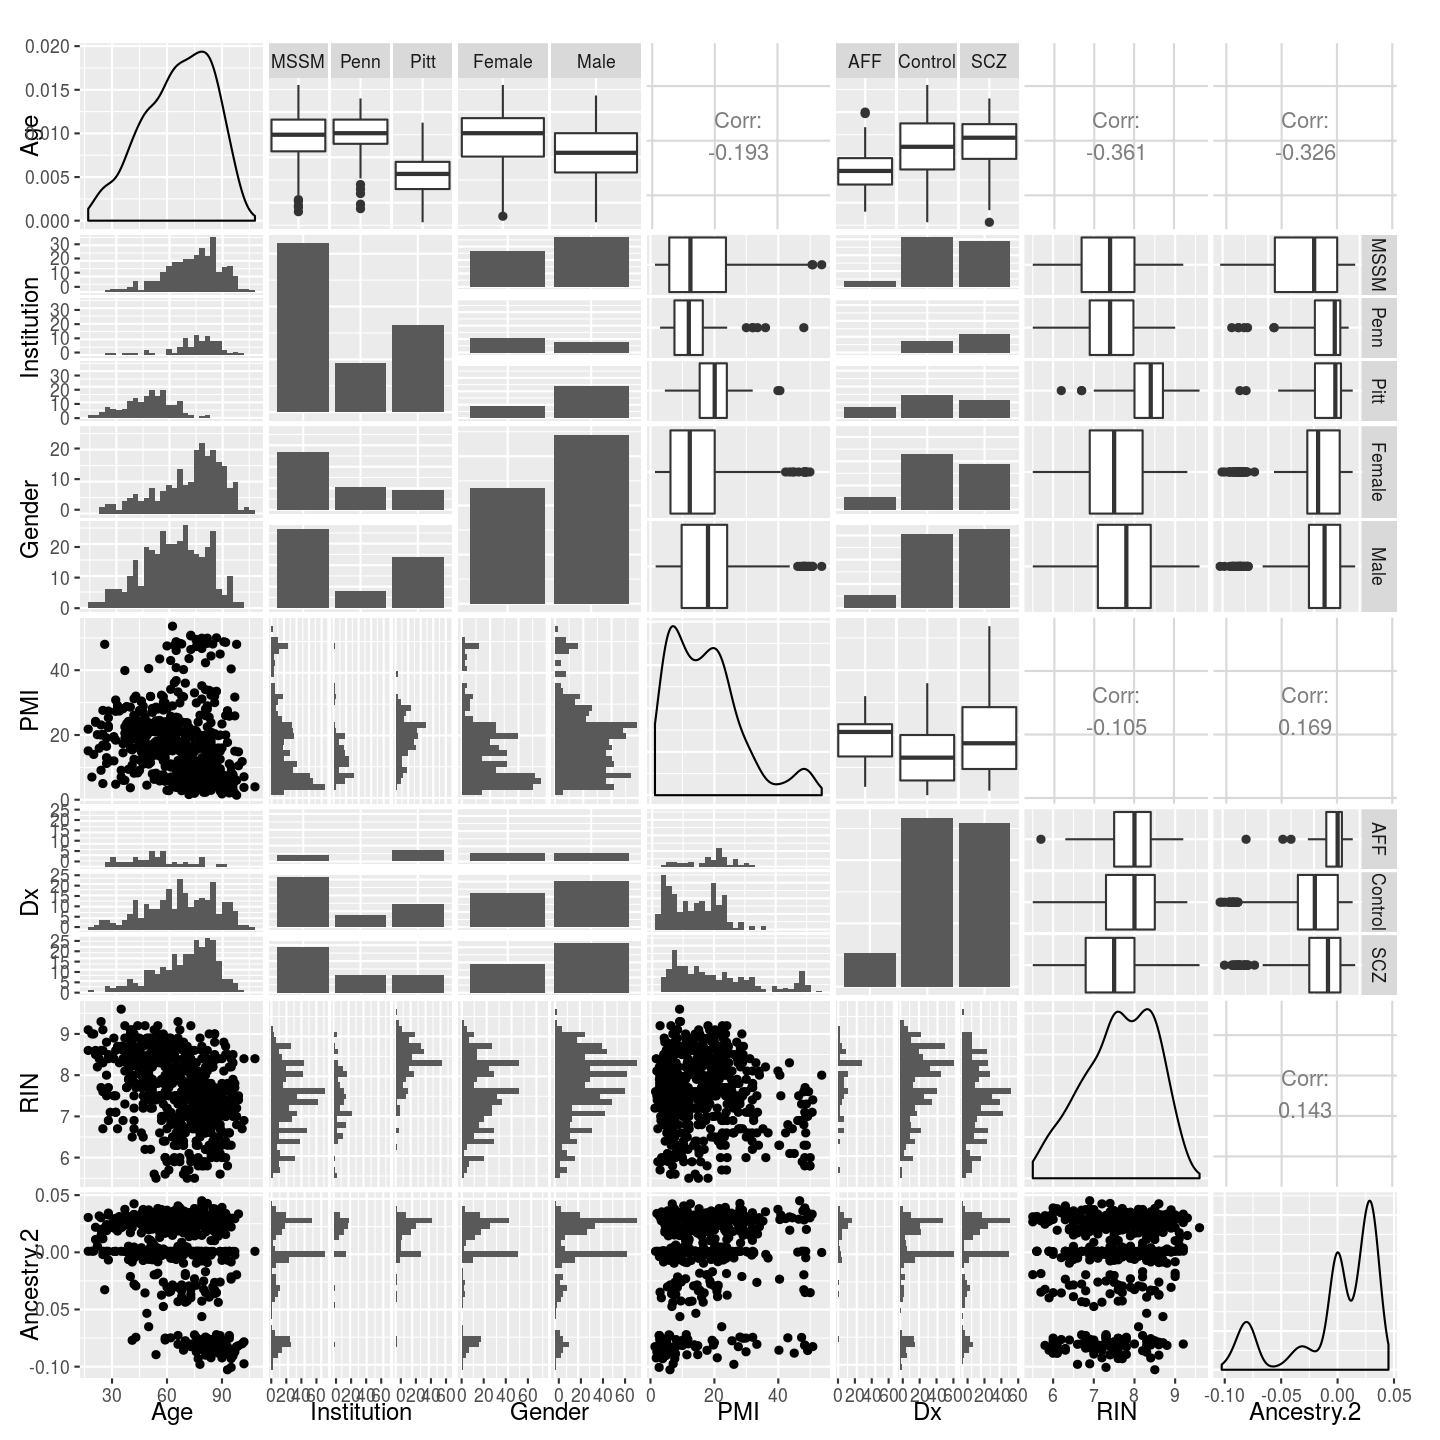
\includegraphics[scale=0.6]{figures/2016-06-26-trellis-display-of-data/evar-scatterplot-matrix-2.png}
\end{center}
\caption{
Distribution and inter-dependence of predictors.  The diagonal graphs of the
plot-matrix show the marginal distribution of six predictors (Age,
Institution,...)~while the off-diagonal graphs show pairwise joint
distributions.  For instance, the upper left graph shows that, in the whole
cohort, individuals' Age
ranges between ca.~15 and 105 years and most individuals around 75 years; the
bottom and right neighbor of this graph both show (albeit in different
representation) the joint distribution of Age and Institution, from which can
be seen that individuals from Pittsburg tended to be younger than those from
the two other institutions.
}
\label{fig:predictor-associations}
\end{figure}

\begin{figure}[h]
\begin{center}
\includegraphics[scale=0.6]{figures/2016-06-26-trellis-display-of-data/S-age-gender-1.png}
\caption{
Variation of the read count ratio \(S_{ig}\) with age and gender across hundreds of individuals
\(i\) (dots) and 30 genes \(g\) that have been considered as imprinted in the DLPFC
brain area in this study.
}
\label{fig:S-age-gender}
\end{center}
\end{figure}

\begin{figure}[h]
\begin{center}
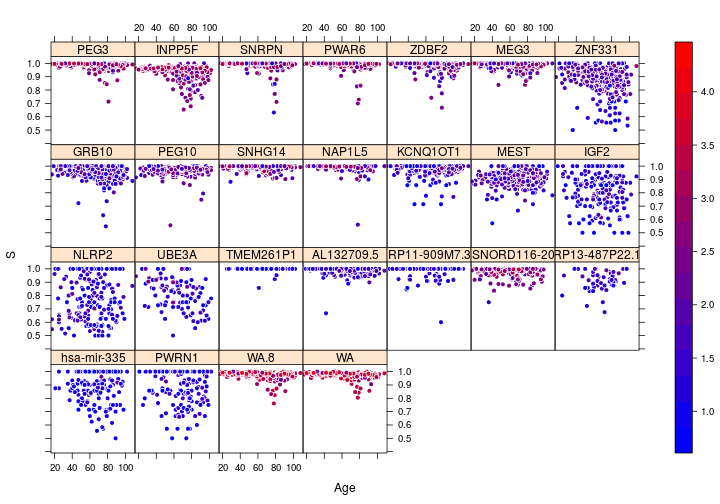
\includegraphics[scale=0.6]{figures/2016-06-26-trellis-display-of-data/S-age-tot-read-count-1.png}
\end{center}
\caption{Variation of total RNA-seq read count across genes and individuals.}
\label{fig:weight-of-evidence}
\end{figure}

\begin{figure}[h]
\begin{center}
\includegraphics[scale=0.6]{figures/2016-09-23-model-checking/qqnorm-wnlm-Q-1.pdf}
\end{center}
\caption{
Checking the fit of wnlm.Q model: analysis of the normality of residuals.
}
\label{fig:qqnorm-wnlm.Q}
\end{figure}

\begin{figure}[h]
\begin{center}
\includegraphics[scale=0.6]{figures/2016-09-23-model-checking/qqnorm-logi-S-1.pdf}
\end{center}
\caption{
Checking the fit of logi.S model: analysis of the normality of standardized deviance residuals.
}
\label{fig:qqnorm-logi.S}
\end{figure}

\begin{figure}[h]
\begin{center}
\includegraphics[scale=0.6]{figures/2016-09-23-model-checking/homoscedas-wnlm-Q-1.pdf}
\end{center}
\caption{
Checking the fit of wnlm.Q model: analysis of homoscedasticity.
}
\label{fig:homoscedas-wnlm.Q}
\end{figure}

\begin{figure}[h]
\begin{center}
\includegraphics[scale=0.6]{figures/2016-09-23-model-checking/homoscedas-logi-S-1.pdf}
\end{center}
\caption{
Checking the fit of logi.S model: analysis of homoscedasticity.
}
\label{fig:homoscedas-logi.S}
\end{figure}

\begin{figure}[h]
\begin{center}
\includegraphics[scale=0.6]{figures/2016-09-23-model-checking/influence-wnlm-Q-1.pdf}
\end{center}
\caption{
Checking the fit of wnlm.Q model: analysis of the impact of outliers.
}
\label{fig:influence-wnlm.Q}
\end{figure}

\begin{figure}[h]
\begin{center}
\includegraphics[scale=0.6]{figures/2016-09-23-model-checking/influence-logi-S-1.pdf}
\end{center}
\caption{
Checking the fit of logi.S model: analysis of the impact of outliers.
}
\label{fig:influence-logi.S}
\end{figure}

\begin{figure}[h]
\begin{center}
\includegraphics[scale=0.6]{figures/2016-10-03-permutation-test/p-val-tdist-vs-perm-filt-iso-1.pdf}
\end{center}
\caption{Agreement between a parametric (t-distribution) and non-parametric
(permutations) method of estimating p-values.}
\label{fig:pval-tdist-vs-perm}
\end{figure}

\begin{figure}[h]
\begin{center}
\includegraphics[scale=0.6]{figures/2016-10-03-permutation-test/p-values-1.pdf}
\end{center}
\caption{
Significance of association between biological predictors and imprinted genes
in the DLPFC calculated under wnlm.Q and logi.S.  Under logi.S, only those
genes are shown for which the model fit was acceptable.
}
\label{fig:pval}
\end{figure}

\begin{figure}[h]
\begin{center}
\includegraphics[scale=0.6]{figures/2016-08-08-imprinted-gene-clusters/segplot-logi-S-99conf-1.pdf}
\end{center}
\caption{
Estimate \(\hat{\beta}_{jg}\) and 99\% confidence interval of each regression coefficient
\(\beta_{jg}\) under the logi.S model, where \(j\) is a predictor/term and
\(g\) is a gene.  \(\hat{\beta}_{jg}\) and the confidence interval are shown only for those
genes are shown for which the model fit was acceptable.
}
\label{fig:biol-effects-logi.S}
\end{figure}

\begin{figure}[h]
\begin{center}
\includegraphics[scale=0.6]{figures/2016-08-21-likelihood-surface/explain-rll-wireframe-1.png}
\includegraphics[scale=0.6]{figures/2016-08-21-likelihood-surface/explain-rll-levelplot-B-1.png}
\end{center}
\caption{
\emph{Top} and \emph{bottom}: two representations of the relative log
likelihood on a 2 dimensional section of the \(p>20\) dimensional parameter
space given the wnlm.Q model and data for the gene \(g=\mathrm{PEG3}\).  The
section was taken by fixing all but two parameters at their estimates:
\(\beta_{jg} = \hat{\beta}_{jg}\).  A rectangular subspace for these two
parameters, \(\beta_{\mathrm{Age},g}\) and  \(\beta_{\mathrm{Ancestry.2},g}\),
was chosen around the maximum likelihood estimate \(\hat{\beta} =
(\hat{\beta}_{\mathrm{Age},g}, \hat{\beta}_{\mathrm{Ancestry.2},g})\).  The
nearly parabolic shape of the log-likelihood function suggests that the
regularity conditions for likelihood-based parametric inference are fulfilled.
}
\label{fig:ll-surf-explain}
\end{figure}

\begin{figure}[h]
\begin{center}
\includegraphics[scale=0.6]{figures/2016-06-22-extending-anova/logi-S-wnlm-Q-compare-1.pdf}
\end{center}
\caption{
Agreement of the wnlm.Q and logi.S models in terms of estimated regression
coefficients.
}
\label{fig:logi.S-wnlm.Q-compare}
\end{figure}

\begin{figure}[h]
\begin{center}
\includegraphics{figures/by-me/monoall-dependencies-2/obs-simple-general/obs-simple-general}
\hspace{\fill}
\includegraphics{figures/by-me/monoall-dependencies-2/obs-simple-general-gene-aspec/obs-simple-general-gene-aspec}
\hspace{\fill}
\includegraphics{figures/by-me/monoall-dependencies-2/obs-bayesian/obs-bayesian}
\end{center}
\caption{ General dependency structure of three regression model frameworks.
In all of threse model frameworks the regression coefficients
\(\beta_{1g},...,\beta_{3g}\) mediate, for a given gene \(g\), probabilistic
dependencies (arrows) between the response variable \(Y_g\) (read count ratio
for \(g\)) and the corresponding predictors \(X_1,...,X_3\).  For simplicity
but without loss of generality only 3 predictors are depicted.  The model
frameworks differ in how \(\beta_{jg_1},\beta_{jg_2},...\) relate to each
other for a given predictor (or a given \(j\)).  \emph{Left:} there is no
connection among \(\beta_{jg_1},\beta_{jg_2},...\) which means that the way
\(Y_{g}\), the read count ratio for gene \(g\) depends on predictor \(X_j\) is
completely separate from how the read count ratio for any other gene \(g'\)
(i.e.~\(Y_{g'}\)) depends on it.  Consequently no information may be shared
among gene-specific models.  \emph{Middle:} In this case
\(\beta_{jg_1}=\beta_{jg_2}=...\equiv\beta_j\) so that all genes are identical
with respect to how their read count ratio depends the predictors.  Thus genes
share all information in the data in the sense that the model forces them to
be identical.  \emph{Right:} Hierarchical Bayesian model where genes show both
variation as well as invariance with regards to depenencies.  The variation is
described by the dependence of \(\beta_j\) on the hyperparameter \(\gamma_j\),
whereas the invariance by the dependence of \(\gamma_j\) on \emph{its}
hyperparameter \(\xi_j\).  Only this model framework allows information
sharing among genes in a flexible way.  }
\label{fig:glm-vs-hierarch}
\end{figure}

\begin{figure}[h]
\begin{center}
\includegraphics[scale=0.6]{figures/2016-06-22-extending-anova/reg-coef-wnlm-Q-1.pdf}
\end{center}
\caption{
Estimates \(\hat{\beta}_{jg}\) and confidence intervals for regression
coefficients under the wnlm.Q model concerning for all predictors.
}
\label{fig:all-effects-wnlm.Q}
\end{figure}

\begin{figure}[h]
\begin{center}
\includegraphics[scale=0.6]{figures/2016-06-22-extending-anova/reg-coef-logi-S-filt-1.pdf}
\end{center}
\caption{
Estimates \(\hat{\beta}_{jg}\) and confidence intervals for regression
coefficients under the logi.S model concerning for all predictors.  Gaps
for certain genes indicate unacceptable fit.
}
\label{fig:all-effects-logi.S}
\end{figure}

\begin{figure}[h]
\begin{center}
\includegraphics[scale=0.6]{figures/2016-08-21-likelihood-surface/ll-surf-coefs-wnlm-Q-1.png}
\end{center}
\caption{
Analysis of orthogonality of regression coefficients.  Relative log-likelihood
surfaces for the gene PEG3 on various rectangles corresponding to 2D sections
through the \(p>20\) dimentional parameter space.  The set of points in a
rectangle where log-likelihood takes the same value are quasi-ellipses, whose
major and minor axes and their tiltedness express association between
coefficients.  For instance, \(\beta_\mathrm{Age}\) is not assiciated with
(orthogonal to) \(\beta_\mathrm{Ancestry.2}\) but is strongly associated with
\(\beta_\mathrm{RIN}\).  Such association hinders statistical inference due to
the following circularity: If we knew the precise value of
\(\beta_\mathrm{RIN}\) we could estimate the true value of
\(\beta_\mathrm{Age}\) with higher precision and confidence but the precise
value of \(\beta_\mathrm{RIN}\) could only be obtained with high confidence if
we precisely knew \(\beta_\mathrm{Age}\).
}
\label{fig:ll-non-orthogonality}
\end{figure}

\begin{figure}[h]
\begin{center}
\includegraphics[scale=0.6]{figures/2016-07-08-conditional-inference/beta-age-cond-wnlm-Q-2-1.pdf}
\end{center}
\caption{
Analysis of interactions among predictors under the wnlm.Q model.  Contextual depenendence of the
read count ratio on age, where the context is given by some specific level of
Institution (MSSM, Penn, Pitt) or Gender (Female, Male).
}
\label{fig:interaction-wnlm.Q}
\end{figure}

\begin{figure}[h]
\begin{center}
\includegraphics[scale=0.6]{figures/2016-07-08-conditional-inference/beta-age-cond-logi-S-2-skip-1.pdf}
\end{center}
\caption{
Analysis of interactions among predictors under the logi.S model.  The missing
panels correspond to genes for which logi.S did not provide acceptable fit.
}
\label{fig:interaction-logi.S}
\end{figure}

\begin{figure}[h]
\begin{center}
\includegraphics[scale=0.6]{figures/2016-06-22-extending-anova/anova-effects-fw-rv-wnlm-Q-1.pdf}
\end{center}
\caption{
\emph{Left:} analysis of variance (ANOVA) is undermined by the non-orthogonality of
predictors because the reduction in deviance (i.e.~in residual sum of squares)
for a term (predictor) depends on the sequence in which terms are added to the
model.  \emph{Right:} the same concept is demonstrated using QR decomposition.
}
\label{fig:anova}
\end{figure}

\begin{figure}[h]
\begin{center}
\includegraphics[scale=0.6]{figures/2016-10-20-differential-expression-scz/venn-triple-1.pdf}
\end{center}
\caption{
Association of genes' expression to schizophrenia (SCZ) assayed by two RNA-seq
based approaches: total read count (overall expression, Nat Neurosci.~2016
Nov;19(11):1442-1453.)~and read count ratio
(allelic bias, present work).  When these approaches are compared for only
those genes that we find imprinted in the DLPFC in this study, 1 gene is found
associated to schizophrenia by both approaches, 1 by only overall expression,
and 3 by only allelic bias.
}
\label{fig:diff-exp-scz}
\end{figure}

%\begin{figure}[h]
%\includegraphics[width=0.6\textwidth]{figures/2016-10-11-comparison-to-mouse-cerebellum/posterior-pp-vs-pval-wnlm-Q-1.pdf}
%\caption{Comparison of the effects of age and gender between the present work and a
%previous study~\cite{Perez2015} in the mouse cerebellum. }
%\label{fig:mouse-cerebellum}
%\end{figure}

\end{document}
